\noindent
\begin{tabular}{cc}
\begin{minipage}[b]{0.60\textwidth}
\begin{exerciseS}
Determinare la portata d'acqua che scorre all'interno del tubo di Venturi 
rappresentato in figura, quando sia trascurabile ogni effetto dissipativo 
all'interno della corrente e la velocit\`{a} uniforme nelle sezioni considerate e
a monte del Venturi.
Dati: densit\`{a} dell'acqua $\overline{\rho}= 999\ kg/m^3$, 
densit\`{a} dell'aria $\overline{\rho}= 1.225\ kg/m^3$,
diametro del tubo $D=2\ cm$, diametro della sezione di gola
$d=1\ cm $, altezze: $z_1 = 10\ cm $, $z_2 = 1.2\ m $,
$z_3 = 5\ cm $, $z_4 = 0.5\ m $.

($Q=3.01\, 10^{-4}\ m/s$, $\overline{Q}=3.005\, 10^{-1}\ kg/s$)
\end{exerciseS}
\end{minipage}
&
\begin{minipage}{0.35\textwidth}
   \begin{center}
   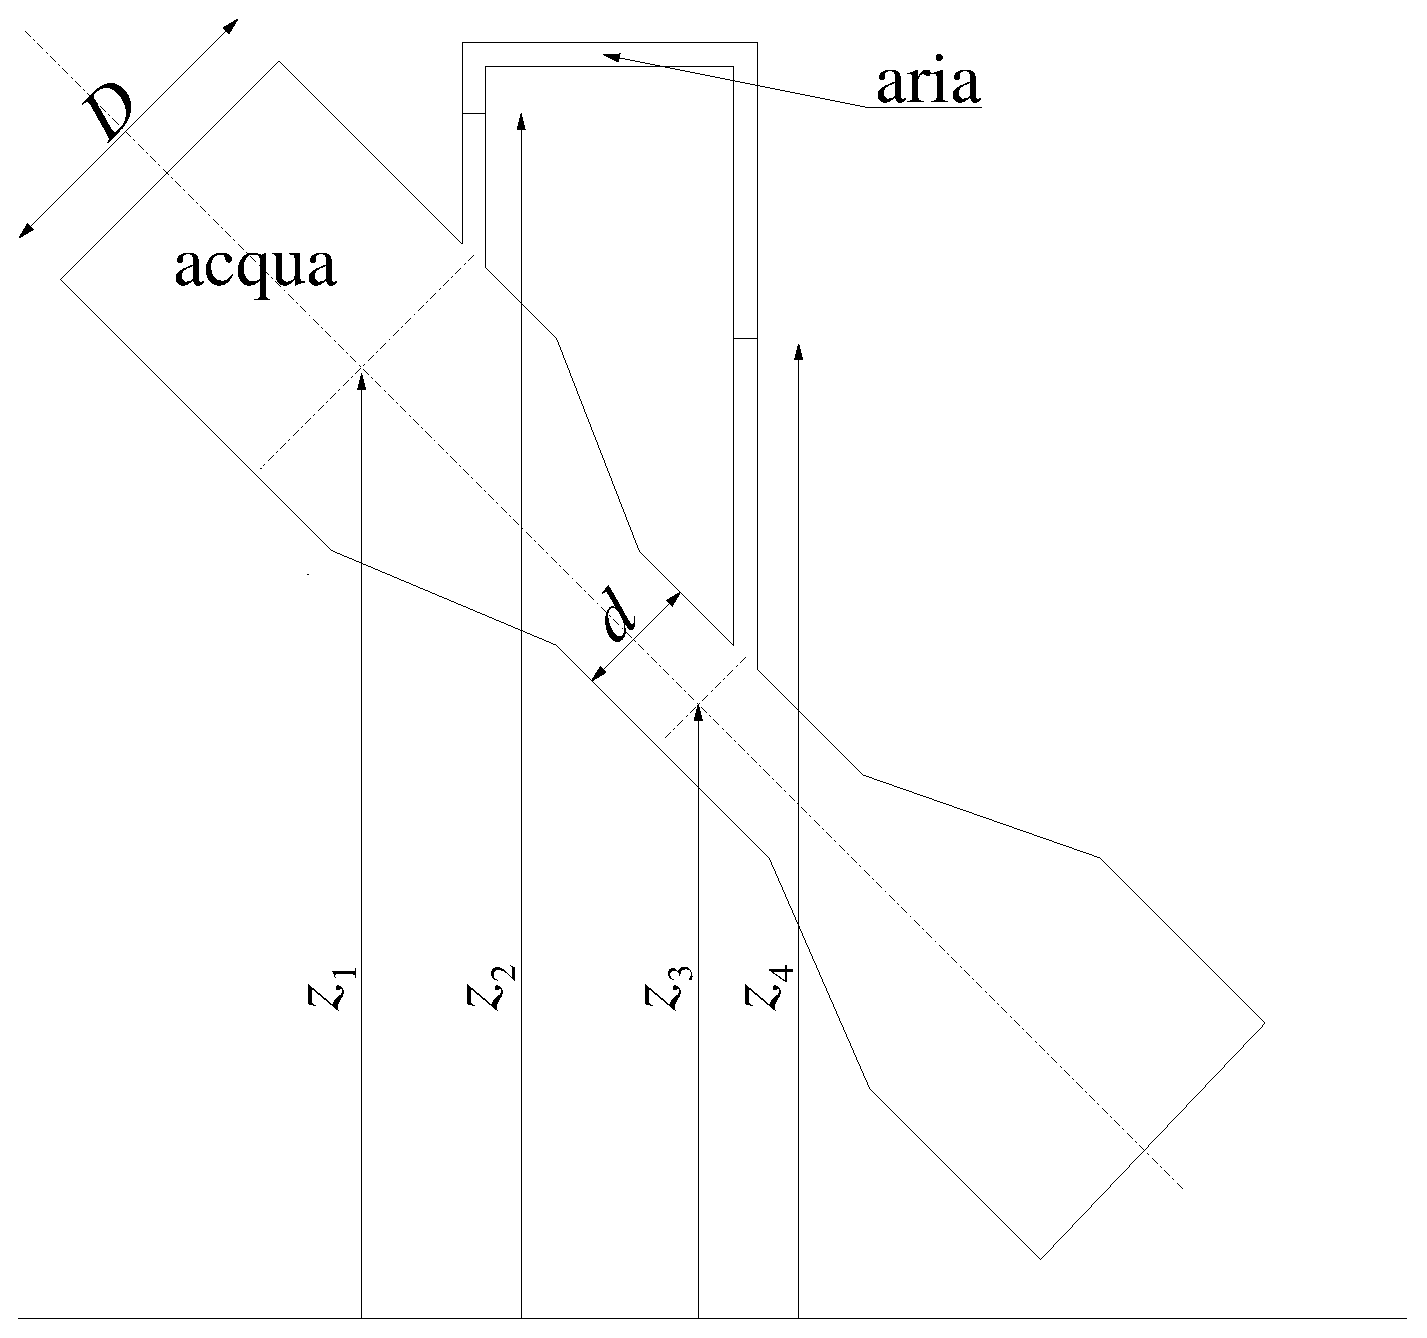
\includegraphics[width=0.90\textwidth]{./fig/venturi.eps}
   \end{center}
\end{minipage}
\end{tabular}

\sol

\partone
Teorema di Bernoulli nell'ipotesi di stazionarietà, fluido incomprimibile, non viscoso, irrotazionale.
Equazione della vorticità nel caso non viscoso.
Legge di Stevino.

\parttwo
Il problema viene risolto con l'applicazione del teorema di Bernoulli (ipotesi...; eq. della vorticità:...) e della continuità all'interno del condotto, e della legge di Stevino all'interno del tubicino.

\begin{equation}
\begin{cases}
 U D^2 = u d^2 & \text{(continuità)} \\
 P_1 + \frac{1}{2}U^2 + \rho g z_1 = P_3 + \frac{1}{2}u^2 + \rho g z_3 & \text{(Bernoulli 1-3)} \\
 P_2 + \rho_a g z_2 = P_4 + \rho_a g z_4 \\
 P_1 + \rho g z_1 = P_2 + \rho g z_2   & \text{(Stevino)} \\
 P_3 + \rho g z_3 = P_4 + \rho g z_4 \\
\end{cases}
\end{equation}

Anche se il numero di equazioni è minori del numero di incognite, prova che il sistema è indeterminato, si dimostra che la $U$ è determinata (nelle equazioni intervengono sempre differenze di pressioni).

Inserendo la $u$ ricavata dalla continuità nel teorema di Bernoulli e risolvendo per $U$:
\begin{equation}
  \frac{1}{2} \rho U^2 (1 - \frac{D^4}{d^4}) = P_3 - P_1 + \rho g (z_3 - z_1)
\end{equation}

Risolvendo per $P_3 - P_1$ le tre equazioni di Stevino, $P_3 - P_1 = - \rho g(z_2-z_1+z_3-z_4) + \rho_a g (z_2 - z_4)$.
E quindi: 
\begin{equation}
  \frac{1}{2} \rho U^2 (1 - \frac{D^4}{d^4}) = g (\rho - \rho_a) (z_2 - z_4) \quad
  \Rightarrow \quad U = \sqrt{\frac{2 g (1 - \rho_a/\rho) (z_2 - z_4)}{1 - \frac{D^4}{d^4}}}
\end{equation}
Le portate sono quindi:
\begin{equation}
 Q = \frac{\pi}{4} D^2 U \quad , \quad \bar{Q} = \rho Q
\end{equation}

Inserendo i valori numerici, si trova: $U = 0.956 m/s$, $Q = 3.0 \cdot 10^{-4} m^3/s$, $\bar{Q} = 3.0 \cdot 10^{-1} kg/s$.
